\chapter{Frontend et Expérience Utilisateur}
\label{chap:frontend}

\section{Architecture Frontend et Paradigme Svelte 5 Runes}

L'application web de Perceptra (\texttt{web/}) repose sur une stack front-end d'avant-garde combinant \textbf{SvelteKit 3} et le moteur de réactivité unifié \textbf{Svelte 5}. Contrairement aux frameworks historiques basés sur un DOM virtuel lourd (Virtual DOM comme React ou Vue), Svelte compile les composants en instructions JavaScript chirurgicales directes, offrant des performances d'affichage optimales indispensables pour manipuler des collections de milliers d'images.

\begin{figure}[H]
\centering
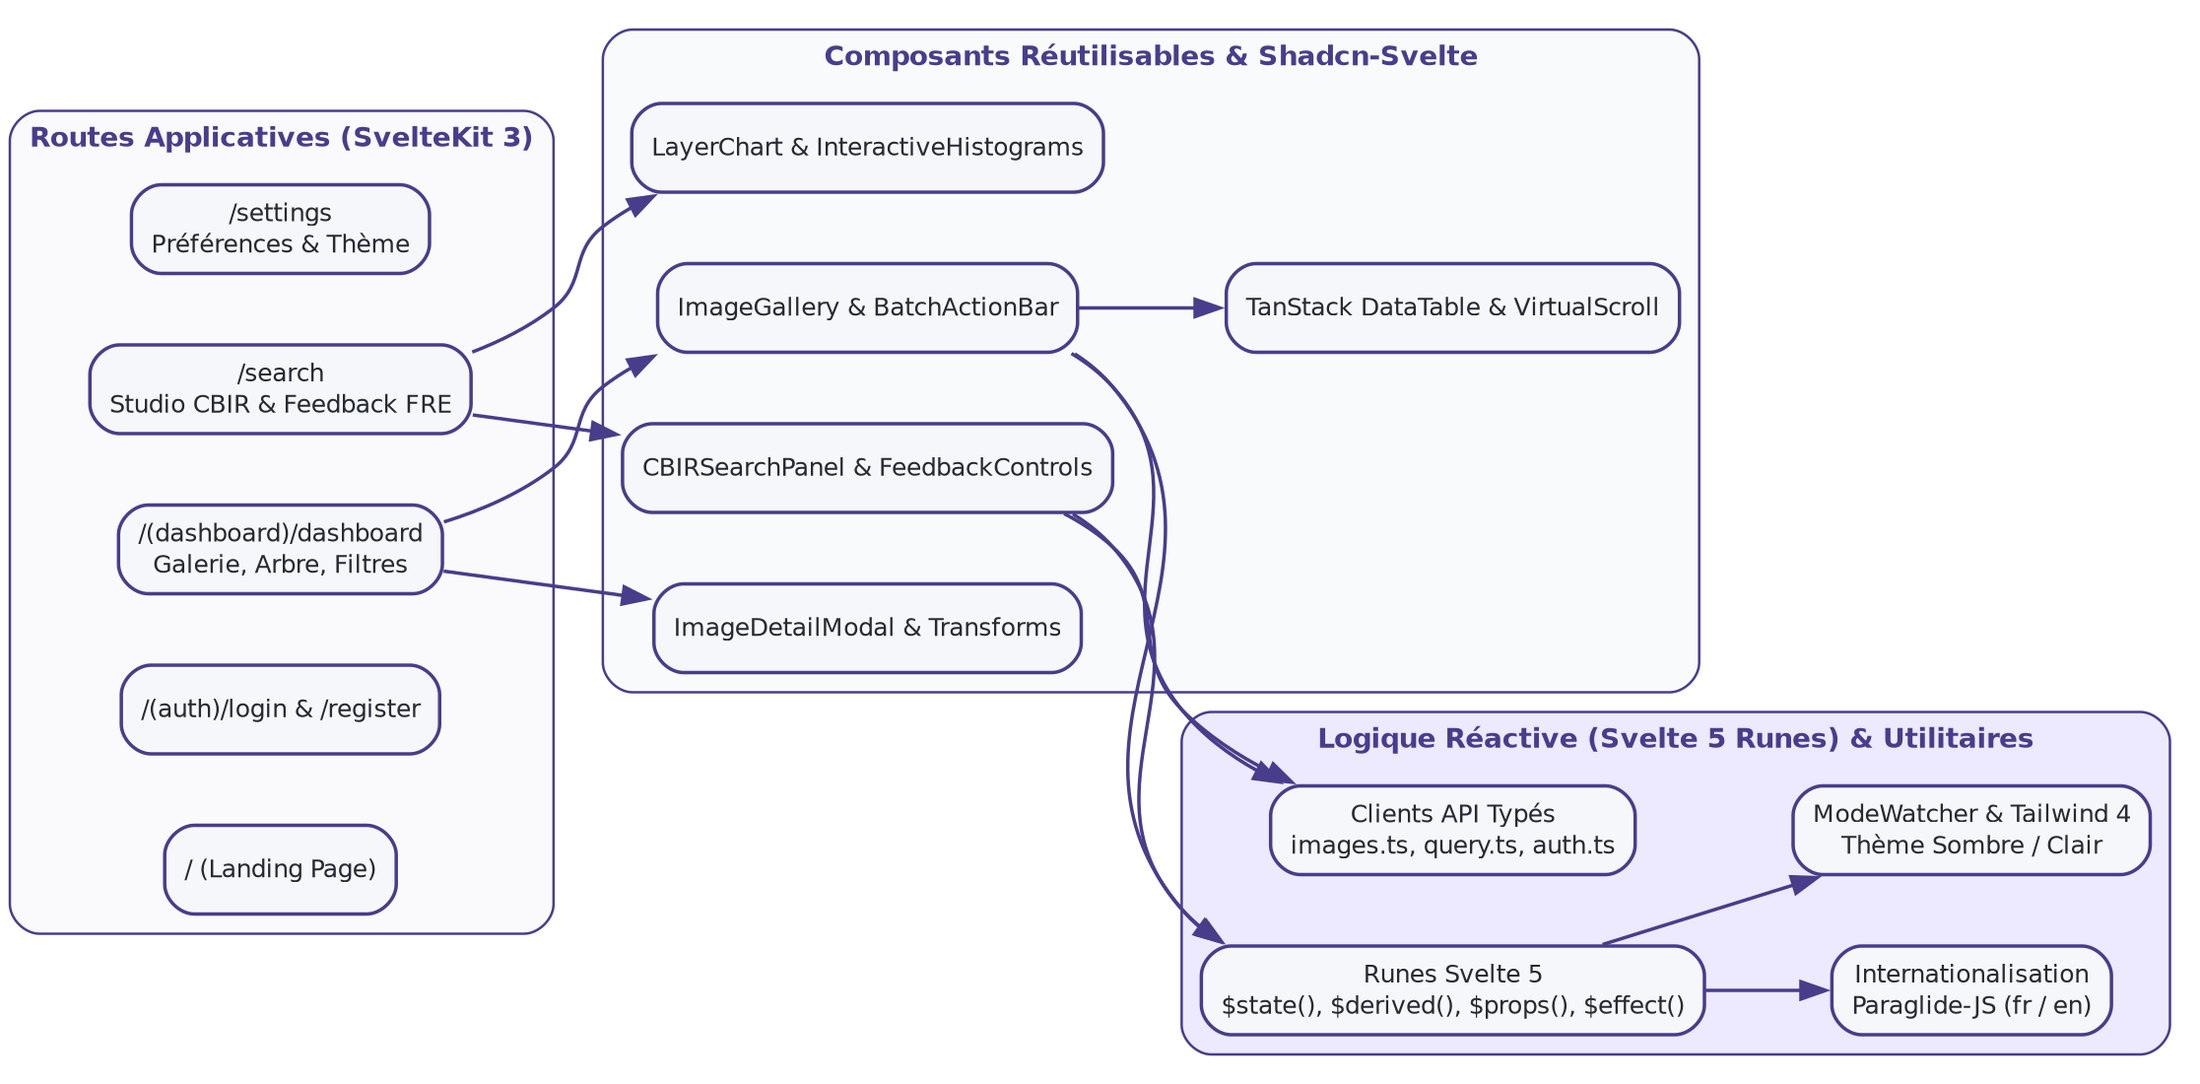
\includegraphics[width=0.78\textwidth]{images/08-architecture-frontend-sveltekit.png}
\caption{Architecture réactive du frontend SvelteKit et organisation des composants}
\label{fig:frontend_arch}
\end{figure}

Le développement exploite exhaustivement les \textbf{Runes} introduites par Svelte~5~:
\begin{itemize}
    \item \texttt{\$state()} : Déclaration explicite des variables d'état réactives (ex: images sélectionnées, filtres actifs, résultats)~;
    \item \texttt{\$derived()} : Calcul automatisé et mémorisé de propriétés dérivées (ex: comptage filtré, somme des poids)~;
    \item \texttt{\$props()} : Déclaration strictement typée des propriétés transmises aux composants enfants via TypeScript~;
    \item \texttt{\$effect()} : Gestion déterministe des effets de bord (synchronisation API, persistance du thème).
\end{itemize}

\section{Système de Conception : Shadcn-Svelte et Tailwind CSS 4}

Pour garantir une identité visuelle professionnelle et accessible, Perceptra intègre la suite de composants \textbf{Shadcn-Svelte} articulée sur les primitives accessibles de \textbf{Bits UI} et stylisée avec le moteur \textbf{Tailwind CSS 4}~:
\begin{itemize}
    \item \textbf{Thématisation Dynamique~:} Prise en charge native du mode sombre et mode clair pilotée par \texttt{mode-watcher}, avec respect strict des contrastes WCAG AAA.
    \item \textbf{Composants Fondamentaux~:} Modales de dialogue (\texttt{Dialog}), volets latéraux contextuels (\texttt{Sheet}), tiroirs coulissants tactiles (\texttt{Drawer} via Vaul-Svelte), menus déroulants et notifications toast instantanées (\texttt{svelte-sonner}).
    \item \textbf{Tableaux de Données Avancés~:} Intégration de \texttt{@tanstack/svelte-table} pour le tri multi-colonnes, la recherche textuelle en temps réel et la pagination virtuelle.
\end{itemize}

\section{Modules Applicatifs et Écrans Principaux}

L'interface de Perceptra s'articule autour de trois espaces majeurs~:

\subsection{1. Galerie de Médias et Organisation (\texttt{/dashboard})}
\begin{itemize}
    \item \textbf{Explorateur Arborescent de Catégories~:} Panneau latéral rétractable affichant l'arbre hiérarchique des dossiers créés par l'utilisateur avec comptage réactif des médias rattachés.
    \item \textbf{Grille Réactive d'Images~:} Affichage adaptatif avec chargement paresseux (\textit{lazy loading}) des vignettes optimisées et statut favori.
    \item \textbf{Barre d'Actions par Lot (\texttt{BatchActionBar})~:} Barre d'action flottante surgissant lors de la sélection multiple pour autoriser la suppression groupée ou l'exportation.
\end{itemize}

\subsection{2. Modale de Retouche et Caractérisation (\texttt{ImageDetailModal})}
Visualiseur exhaustif des caractéristiques physiques et atelier complet de transformation non destructive~: recadrage avec règle des tiers, curseurs de redimensionnement proportionnel et rotations libres.

\subsection{3. Studio de Recherche CBIR et Rétroaction (\texttt{/search})}
\begin{enumerate}
    \item \textbf{Dépôt de la Requête Visuelle~:} Glisser-déposer d'une image locale ou sélection dans la galerie.
    \item \textbf{Panneau de Configuration des Poids~:} Curseurs ergonomiques pour doser l'influence relative de chaque descripteur.
    \item \textbf{Grille de Résultats Ordonnés~:} Restitution instantanée des $K$ images les plus proches avec badges de similarité globale, chromatique et texturale.
    \item \textbf{Contrôles de Pertinence et FRE~:} Bouton vert (Pertinent) et bouton rouge (Non-pertinent). Le bouton «~Réestimer la pertinence (FRE)~» déclenche l'ajustement adaptatif et le réordonnancement de la collection.
\end{enumerate}

\section{Visualisations Analytiques et Internationalisation Bilingue}

Perceptra intègre la bibliothèque \textbf{LayerChart} et \textbf{D3.js} pour restituer les histogrammes spectro-chromatiques sous forme de barres SVG colorées et tracer l'évolution des poids FRE. L'internationalisation est assurée par \textbf{Paraglide-JS}, garantissant un bilinguisme intégral (Français/Anglais) compilé statiquement avec vérification TypeScript à zéro surcharge d'exécution.
